\documentclass[12pt, a4paper]{article}%Tipo de documento y tamaño de letra%
\usepackage[spanish]{babel}
\usepackage{color,graphicx}%Para poder insertar graficas%
\usepackage{graphics}
\usepackage{minted}
\usepackage{amsmath,amssymb}%Insertar unos símbolos matemáticos especiales%
%%%%%%%%%%%%%%%% LA INTEGRAL COMEMIERDA ESA%%

\def\Xint#1{\mathchoice
{\XXint\displaystyle\textstyle{#1}}%
{\XXint\textstyle\scriptstyle{#1}}%
{\XXint\scriptstyle\scriptscriptstyle{#1}}%
{\XXint\scriptscriptstyle\scriptscriptstyle{#1}}%
\!\int}
\def\XXint#1#2#3{{\setbox0=\hbox{$#1{#2#3}{\int}$ }
\vcenter{\hbox{$#2#3$ }}\kern-.6\wd0}}
\def\ddashint{\Xint=}
\def\dashint{\Xint-}

%%%%%%%%%%%%%%%%%%%%%%%%%%%%%%%%%%%%%%%%%%%%

\usepackage{silence}
\WarningFilter{latexfont}{Font shape `T1/ntxtlf/m/up' undefined}
\WarningFilter{latexfont}{Some}
\usepackage{setspace}
%\usepackage{empheq}
\usepackage{multicol}
\usepackage[most]{tcolorbox}
\usepackage{lipsum}
\usepackage{mathrsfs}
\usepackage[T1]{fontenc}
\usepackage{newtxtext,euler}
\let\oldstylenums\oldstyle
\usepackage{array}
\usepackage{layout}
\usepackage{manfnt}
\usepackage{float}
\usepackage{xcolor}
\usepackage{tcolorbox}
\usepackage{lipsum}
\usepackage{tikz}
\usepackage{amsthm}
\usepackage{enumerate}
\usepackage{picinpar}
% Tcolorboxes

\makeatother
\usepackage{thmtools}
\usepackage[framemethod=TikZ]{mdframed}
\mdfsetup{skipabove=1em,skipbelow=1em}

\newcommand{\sqed}{\hfill
\includegraphics[height=2ex]{sancoya.png}}

\theoremstyle{definition}
\declaretheoremstyle[
    headfont=\bfseries\sffamily\color{black!70!black}, bodyfont=\normalfont,
    mdframed={
        linewidth=2pt,
        rightline=false,leftline=false, topline=false, bottomline=false,
        linecolor=black, backgroundcolor=black!2!white,
    }
]{thmbox}

\declaretheoremstyle[
    headfont=\bfseries\sffamily\color{black!70!black}, bodyfont=\normalfont,
    numbered=no,
    mdframed={
        linewidth=0pt,
        rightline=false, topline=false, bottomline=false,
        linecolor=black, backgroundcolor=black!2!white,
    },
    qed=\qedsymbol
]{thmproofbox}

\declaretheoremstyle[
    headfont=\bfseries\sffamily\color{black!70!black}, bodyfont=\normalfont,
    numbered=no,
    mdframed={
        linewidth=0pt,
        rightline=false, topline=false, bottomline=false,
        linecolor=black, backgroundcolor=black!2!white,
    },
]{sancoya}


\declaretheorem[style=thmbox, name=Definición]{definition}
\declaretheorem[style=thmbox, numbered=no, name=Ejemplo]{eg}
\declaretheorem[style=sancoya, numbered=no, name=Demostración]{sproof}
\declaretheorem[style=thmbox, name=Proposición]{prop}
\declaretheorem[style=thmbox, name=Teorema, numbered=no]{theorem}
\declaretheorem[style=thmbox, name=Lema]{lemma}
\declaretheorem[style=thmbox, numbered=no, name=Corolario]{corollary}
\declaretheorem[style=thmbox, name=Solución, numbered=no]{solution}


\declaretheorem[style=thmproofbox, name=Demostración]{replacementproof}
\renewenvironment{proof}[1][\proofname]{\vspace{-10pt}\begin{replacementproof}}{\end{replacementproof}}


\declaretheorem[style=thmbox, numbered=no, name=Nota]{note}
\declaretheorem[style=thmbox, numbered=no, ]{temp}




\usepackage{geometry}
 \geometry{
 a4paper,
 total={170mm,245mm},
 left=25mm,
 top=30mm,
 }

\usepackage{bbm}

\begin{document}

\setlength{\parindent}{0cm}
\hoffset-0.46cm
\voffset-1.46cm

\begin{window}[0,l,{
\includegraphics[scale=0.31]{logo.eps}},]
\large\scshape  \hspace{0.4cm}\textsf{Universidad Nacional de Colombia} \\
\textcolor{white}{\tiny.}  \large \hspace{1.5cm} \textsf{Facultad de Ciencias} \\
\textcolor{white}{\tiny.}   \normalsize\hspace{2.2cm}\textsf{Análisis Numérico I}\\
 

\end{window}

\vspace{0.2cm}
\small
\textsf{Mateo Andrés Manosalva Amaris\\
Edgar Santiago Ochoa Quiroga\\
Sergio Alejandro Bello Torres} 
\normalsize
\dotfill
\vspace{0.7cm}

%Ella a mí siempre me trasnocha, yo la pienso a toda hora, pasa por su casa bien sola, deseo que ella sea mi esposa, y anoche yo me presenté en su casa, le dije to' lo que ella a mí me gustaba, ella me dijo "ay papi, qué bonito, échate pa' acá un poquito". Se me fue acercando poco a poquito, con la primera cita ella me dio un besito, me dijo que fuéramos noviecitos y le quité el shorcito. Y la encendí a mondá en la sala de su casa y terminamos en la terraza, yo le pegué su mondaquera en la cama, esa muchacha como gritaba.%
\section*{Problemas}

\subsection*{Problema1}
Un bloque de masa \( m \) desliza bajo la acción de la gravedad por un plano inclinado formando un ángulo \( \theta \) respecto de la horizontal. Se puede demostrar que, si la fuerza de rozamiento \( F_r \) entre el bloque y el plano viene dada por \( F_r = -k m v^2 \) con \( v \) la velocidad del bloque y \( k \) un coeficiente de rozamiento, entonces el tiempo \( T \) requerido para que el bloque recorra una distancia \( D \) partiendo del reposo está relacionado de la forma
\[
e^{kD} = \cosh\left(T \sqrt{k g \sin \theta}\right),
\]
siendo \( g = 9.8 \) la aceleración de la gravedad. Si \( \theta = \frac{\pi}{4} \), \( k = 0.5 \pm 0.1 \) y \( T = 2 \pm 0.2 \), hallar la precisión con la que se conoce \( D \).
\begin{solution}
    Despejando D de la ecuación, se tiene que:
    \[ D=\frac{\ln{\left(\cosh{\left(T\sqrt{kg\sin{\theta}}\right)}\right)}}{k}
    \]
    Empezaremos asumiendo que el error de cómputo es despreciable, debido a la cantidad de cifras significativas que reporta la calculadora (10 cifras), en contraste con los datos que tenemos, que tienen a lo más dos cifras significativas. De modo que el error podemos obtenerlo de la ecuación:
    \begin{align*}
    \text{Error total}&\approx f(\widehat{x})-f(x)\\
    \intertext{donde}\\ f(x)=f(T,k)&=\frac{\ln{\left(\cosh{\left(T\sqrt{kg\sin{\theta}}\right)}\right)}}{k}
    \end{align*}
    
    Tomando $x=(T,k)$ donde $T=2$ y $k=0.5$; y $\widehat{x}=(\widehat{T},\widehat{k})$ con $\widehat{T}=2+0,2=2,2$ y $\widehat{k}=0,5+0,1=0,6$, conociendo además que $\sin\left(\dfrac{\pi}{4}\right)=\dfrac{\sqrt{2}}
    {2}$, procedemos a calcular $f(T,k)$ y $f(\widehat{T},\widehat{k})$:
    \begin{align*}
        f(T,k)&=\frac{\ln{\left(\cosh{\left(2\sqrt{0,5*9,8*\frac{\sqrt{2}}{2}}\right)}\right)}}{0,5}\approx 6,060487548\\
        f(\widehat{T},\widehat{k})&=\frac{\ln{\left(\cosh{\left(2,2\sqrt{0,6*9,8*\frac{\sqrt{2}}{2}}\right)}\right)}}{0,6}\approx 6,321539517
    \end{align*}

    De esta manera, el error absoluto obtenido al calcular D es:
    \[
    E_{abs}=|6,321539517-6,060487548|=0,261051969
    \] Para hallar la precisión con la que se conoce D, procedemos a calcular el error relativo:
    \[
    E_{rel}=\dfrac{E_{abs}}{|f(x)|}=\dfrac{0,261051969}{6,060487548}=0,04307441719
    \]
    
    De esta manera obtenemos que $E_{rel}\approx 4,31*10^{-2}<5*10^{-2}$, lo cual significa que solo podemos conocer D con una precisión de una cifra significativa.

    \end{solution}
\subsection*{Problema2}
Utilizando el método de redondeo.

\begin{itemize}
    \item[(a)] Hallar el número de máquina más próximo a 125.6 y a 126 si trabaja con
    \begin{itemize}
        \item Base 10 y mantisa de 2 dígitos.
        \item Base 2 y mantisa de 8 dígitos.
    \end{itemize}

    \item[(b)] Verificar para \( x = 125.6 \) la cota para el error relativo
    \[
    \left|\frac{x - \text{fl}(x)}{x}\right| \leq \epsilon
    \]
    si \( \epsilon = \frac{1}{2} \beta^{1-d} \) donde \( \beta \) es la base y \( d \) la longitud de la mantisa.

    \item[(c)] ¿Cuál es, en cada caso, el valor que da la máquina como resultado de las operaciones \( 126 + 126.5 \) y \( 126 - 125.6 \)? ¿Cuál es el error relativo de estos resultados?
\end{itemize}

\subsection*{Problema3}
Suponga que una compañía de computadores está desarrollando un nuevo sistema de punto flotante para usarlo con sus máquinas. Ellos necesitan su ayuda para responder unas preguntas acerca de su sistema. Siguiendo la terminología descrita en clase, el sistema de punto flotante de la compañía se especifica por \( (\beta, t, L, U) \). Usted debe suponer que:

\begin{itemize}
    \item Todos los valores de punto flotante son normalizados (excepto la representación de punto flotante de cero).
    \item Todos los dígitos en la mantisa de un valor de punto flotante son almacenados explícitamente.
    \item El cero se representa con una mantisa y exponente de ceros.
\end{itemize}

Preguntas:
\begin{itemize}
    \item[(a)] ¿Cuántos valores diferentes de punto flotante no negativos pueden representarse por medio de este sistema de punto flotante?
    \item[(b)] La misma pregunta para el caso \( (\beta, t, L, U) = (8, 5, -100, 100) \), el cual la compañía está contemplando en particular.
    \item[(c)] ¿Cuál es el valor aproximado (en base 10) del número más grande y el número positivo más pequeño que pueden ser representado en este sistema de punto flotante?
    \item[(d)] Para el caso general, demuestre que los errores relativos producidos por realizar truncamiento y redondeo son
    \[
    \left|\frac{\text{fl}(x) - x}{x}\right| = 
    \begin{cases}
        \beta^{1-t} & \text{cuando se efectúa truncamiento}, \\
        \frac{1}{2} \beta^{1-t} & \text{cuando se efectúa redondeo}.
    \end{cases}
    \]
\end{itemize}

\subsection*{Problema4}
Considere la expansión de Taylor para la función exponencial
\[
e^x = 1 + x + \frac{x^2}{2!} + \frac{x^3}{3!} + \dots = \sum_{i=0}^{\infty} \frac{x^i}{i!} = \lim_{N \to \infty} S(x, N)
\]
donde \( S(x, N) \) es la suma parcial con \( N + 1 \) términos.

\begin{itemize}
    \item[(a)] Escriba un programa que grafique el error relativo de la suma, \( \dfrac{|S(x, N) - e^x|}{e^x} \) versus \( N \) (hasta \( N = 60 \)) para un valor dado de \( x \). Pruebe su programa para \( x = 10, 2, -2 \) y \( -10 \). De las gráficas, explique por qué ésta no es una buena manera para evaluar \( e^x \) cuando \( x < 0 \).
    \item[(b)] Modifique su programa tal que use la identidad \( e^x = \dfrac{1}{e^{-x}} = \dfrac{1}{S(-x, \infty)} \) para evaluar la función exponencial cuando \( x \) es negativa. Explique por qué esta técnica funciona mejor.
\end{itemize}

\subsection*{Problema5}
\begin{itemize}
    \item[(a)] De manera similar a la desarrollada en clase, deduzca que una aproximación de \( f'(x_0) \) es
    \[
    \dfrac{f(x_0 + h) - f(x_0 - h)}{2h}.
    \]
    Muestre que esta aproximación tiene un error de \( O(h^2) \). Más precisamente, el primer término del error es \( -\dfrac{h^2}{6} f'''(x_0) \) cuando \( f'''(x_0) \neq 0 \).

\begin{proof}
Por el teorema de Taylor tenemos que

$$
f\left(x_0+h\right)=f\left(x_0\right)+h f^{\prime}\left(x_0\right)+\frac{h^2}{2}  f^{\prime \prime}\left(x_0\right)+\frac{h^3}{6} f^{\prime \prime \prime}\left(x_0\right)+\cdots,
$$

además
    
$$
f\left(x_0-h\right)=f\left(x_0\right)-h f^{\prime}\left(x_0\right)+\frac{h^2}{2}  f^{\prime \prime}\left(x_0\right)-\frac{h^3}{6} f^{\prime \prime \prime}\left(x_0\right)+\cdots,
$$

luego el error de aproximación de $f^{\prime}\left(x_0\right)$ por la expresión planteada no considera los términos pares de la expansión de Taylor ya que tienen el mismo signo y se cancelan al realizar la resta como sigue

$$
f\left(x_0+h\right)-f\left(x_0-h\right)=2 h f^{\prime}\left(x_0\right)+\frac{h^3}{6} f^{\prime \prime \prime}\left(x_0\right)+\frac{h^3}{6} f^{\prime \prime \prime}\left(x_0\right)+O(h^5),
$$

así

$$
\begin{aligned}
\frac{f\left(x_0+h\right)-f\left(x_0-h\right)}{2 h} & =f^{\prime}\left(x_0\right)+\frac{ 2h^3}{2h6} f^{\prime \prime \prime}\left(x_0\right)+\cdots \\
& =f^{\prime}\left(x_0\right)+\frac{h^2}{6} f^{\prime \prime \prime}\left(x_0\right)+\cdots,
\end{aligned}
$$

se sigue que


$$\left|\frac{f\left(x_0+h\right)-f\left(x_0-h\right)}{2 h}-f^{\prime}(x_0)\right|\leq \frac{h^2}{6} f^{\prime \prime \prime}\left(x_0\right)+O(h^4)$$

\end{proof}
    
    \item[(b)] Adapte el programa de Matlab hecho en clase para visualizar el comportamiento del error de aproximación a medida que el paso \( h \) decrece desde \( h = 10^{-1}, \dots, 10^{-16} \).

\begin{solution}
        Implementamos el siguiente código:

    \begin{minted}[linenos, fontsize=\small]{matlab}
x0 = 1.2;       
f0 = sin(x0);       
fp = cos(x0);     
i = -16:0.5:-1;
h = 10.^i;
err_centrada = abs(fp - (sin(x0 + h) - sin(x0 - h)) ./ (2 * h));
d_err_centrada = fp / 6 * h.^2;
loglog(h, d_err_centrada, 'r-.', h, err_centrada, 'b-*', 'LineWidth', 2);
xlabel('h', 'fontsize', 16);
ylabel('Error Absoluto', 'fontsize', 14);
legend('Error de truncamiento', 'Diferencias finitas', 'location', 'southwest');
grid on;
\end{minted}

con lo que obtuvimos la gráfica

\begin{figure}[H]
    \centering
    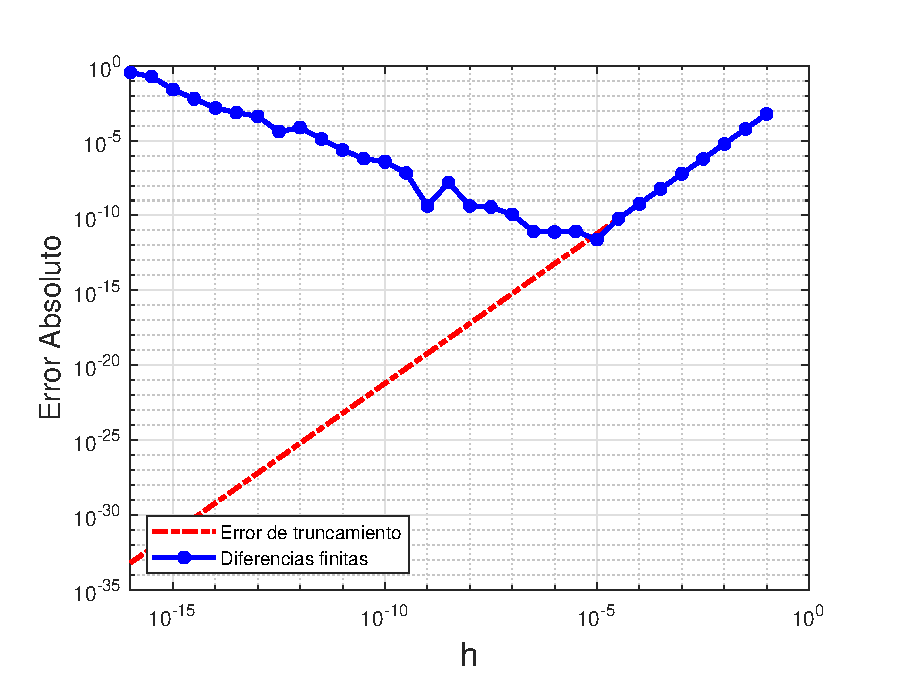
\includegraphics[width=0.75\linewidth]{Gráficas/P5-1.eps}
    \caption{P5-1}
    \label{fig:bluelabel}
\end{figure}
    
\end{solution}

    \item[(c)] Muestre que
    \[
    f'(x_0) = \dfrac{-f(x_0 + 2h) + 8f(x_0 + h) - 8f(x_0 - h) + f(x_0 - 2h)}{12h} + O(h^4)
    \]
    De nuevo adapte su programa para visualizar el comportamiento del error de aproximación a medida que el paso \( h \) decrece desde \( h = 10^{-1}, \dots, 10^{-16} \).
\end{itemize}

\begin{proof}
    De manera análoga al numeral a) tenemos que
    
$$
8f\left(x_0+h\right)-8f\left(x_0-h\right)=16 h f^{\prime}\left(x_0\right)+16\frac{h^3}{6} f^{\prime \prime \prime}\left(x_0\right)+O(h^5),
$$

por otro lado

$$\begin{aligned}
 -&f(x_0+2 h)=-f\left(x_0\right)-2h f^{\prime}\left(x_0\right)-\frac{4 h^2}{2} f^{\prime \prime}\left(x_0\right)-\frac{8 h^3}{6} f^{\prime \prime}\left(x_0\right)+O\left(h^5\right),\\
& f(x_0-2 h)=f\left(x_0\right)-2 h f^{\prime}\left(x_0\right)+\frac{4 h^2}{2}f^{\prime\prime}(x_0)-\frac{8 h^3}{6} f^{\prime \prime \prime}\left(x_0\right)+O\left(h^5\right),
\end{aligned}
$$

sumando estas expresiones obtenemos que 

$$8f\left(x_0+h\right)-8f\left(x_0-h\right)-f(x+2h)+f(x_0+2h)=12hf^{\prime}(x_0)+O(h^5).$$

En efecto 

\begin{align*}
     \dfrac{-f(x_0 + 2h) + 8f(x_0 + h) - 8f(x_0 - h) + f(x_0 - 2h)}{12h}&=\dfrac{12hf^{\prime}(x_0)+O(h^5)}{12h}\\
     =f^{\prime}(x_0)+O(h^4)
\end{align*}

\end{proof}
\subsection*{Problema6}
Repaso de notación \( O \) mayúscula y \( o \) minúscula de una función. Si \( f(x) = O(x^2) \), \( g(x) = O(x^3) \) y \( h(x) = O(x^3) \) cuando \( x \to 0 \), ¿cuáles de las siguientes afirmaciones son verdaderas? Justifique sus respuestas.

\begin{itemize}
    \item[(a)] \( f(x) = o(x) \) cuando \( x \to 0 \)
    \item[(b)] \( f(x) = o(x^2) \) cuando \( x \to 0 \)
    \item[(c)] \( f(x) \cdot g(x) = O(x^5) \) cuando \( x \to 0 \)
    \item[(d)] \( f(x) + g(x) = O(x^3) \) cuando \( x \to 0 \)
    \item[(e)] \( g(x) - h(x) = 0 \)
    \item[(f)] \( \dfrac{g(x)}{h(x)} = O(1) \) cuando \( x \to 0 \)
\end{itemize}
\end{document}

